% MNRAS manuscript. Build on Overleaf (template "Monthly Notices of the RAS")
% or locally with the mnras.cls class:  latexmk -pdf mnras_paper.tex
% Requires mnras.cls + mnras.bst (https://www.ras.ac.uk/, or Overleaf template).
\documentclass[fleqn,usenatbib]{mnras}

\usepackage{newtxtext,newtxmath}
\usepackage[T1]{fontenc}
\usepackage{graphicx}
\usepackage{amsmath}
\usepackage{booktabs}

\newcommand{\msun}{\ensuremath{\mathrm{M}_\odot}}
\newcommand{\phione}{\ensuremath{\phi_1}}
\newcommand{\phitwo}{\ensuremath{\phi_2}}

\title[Subhalo-impact detection in stellar streams]{A reproducible pipeline for
dark-matter subhalo-impact detection in Milky Way stellar streams: a timeline
forward model and an honest current-data limit}

\author[D. W. et al.]{%
D. W.$^{1}$\thanks{E-mail: dwthegreat2@gmail.com}
\\
$^{1}$Independent researcher
}

\date{Accepted XXX. Received YYY; in original form ZZZ}
\pubyear{2026}

\begin{document}
\label{firstpage}
\maketitle

\begin{abstract}
Dark-matter subhalos below the threshold of galaxy formation ($\lesssim10^{8}\,\msun$)
are a key prediction of cold dark matter (CDM) and a discriminator against warm
(WDM), fuzzy (FDM), and self-interacting (SIDM) alternatives. Their gravitational
flybys imprint density gaps and kinematic ripples on thin Milky Way stellar
streams. We present an end-to-end, reproducible pipeline that (i) generates
stream simulations with literature-anchored progenitor orbits, (ii) trains a
graph neural network (GNN) detector with simulation-based inference (SBI), and
(iii) introduces a \emph{timeline forward model} that, given a candidate impact,
estimates its epoch, rewinds the stream, re-injects a grid of encounters with
\citet{ErkalBelokurov2015} impulse physics, re-evolves to the present, and scores
each hypothesis against the observed stream using fused multi-epoch/multi-survey
kinematics. Applying the pipeline to seven streams (GD-1, Pal~5, Orphan--Chenab,
ATLAS, Jhelum, Fj\"orm, Sylgr) with public Gaia DR3, S$^5$, and APOGEE data, we
find \textbf{no joint detection} (Fisher $p=0.30$; Stouffer $p=0.16$), consistent
with a smooth null / CDM and best read as an upper limit given the residual
simulation-to-observation gap. We further show that a detector that appears strong
on a balanced training set (AUC~$0.94$) is only marginally better than chance
(AUC~$0.62$) on physically-faithful simulations, a cautionary result on dataset
construction. Our principal contributions are methodological: a diagnosis and
partial closure of the simulation-to-observation gap, a look-elsewhere--corrected
significance framework with a cross-stream coherence gate, and a public,
test-covered codebase.
\end{abstract}

\begin{keywords}
dark matter -- Galaxy: halo -- Galaxy: kinematics and dynamics -- methods: statistical
\end{keywords}

\section{Introduction}
\label{sec:intro}
The abundance of low-mass dark-matter (DM) subhalos is one of the sharpest
predictions distinguishing CDM from WDM, FDM, and SIDM. Below the threshold of
galaxy formation ($\lesssim10^{8}\,\msun$) these subhalos host no stars, so they
can only be found through their gravity. Thin, dynamically cold stellar streams
--- the tidal debris of disrupted globular clusters and dwarf galaxies --- are
among the most sensitive available probes: a subhalo flyby imprints a density gap,
an off-track spur, and a characteristic kinematic ripple whose morphology encodes
the perturber's mass and impact geometry
\citep{Carlberg2012,ErkalBelokurov2015}. The GD-1 stream in particular shows a
gap-and-spur feature interpreted as dynamical evidence for a dark substructure
\citep{Bonaca2019}, and population-level analyses have begun to place
particle-physics constraints on the subhalo mass function \citep{Banik2021}.

Turning these signatures into a measurement is hard for two reasons. First, gaps
are degenerate: a subhalo impact must be distinguished from baryonic perturbers
(giant molecular clouds, the bar, spiral arms), epicyclic density variations, and
survey systematics. Second, the forward model is expensive, making classical
likelihood-based inference over many hypotheses costly.

We address both with machine learning and simulation-based inference (SBI). A GNN
with edge-conditioned convolutions \citep{Hu2020gine} respects the permutation
symmetry of a member-star set and the locality of kinematic perturbations,
producing an embedding that SBI \citep{Greenberg2019snpe,Tejero-Cantero2020sbi}
maps to a posterior over mass-function parameters, amortizing inference across the
expensive simulator.

Our central methodological idea is a \emph{timeline forward model}. Rather than
classifying only a present-day snapshot, we hypothesize a specific impact, use a
detector to localize and time it, run the clock backward to the unperturbed
stream, re-inject a grid of candidate encounters with the
\citet{ErkalBelokurov2015} impulse, re-evolve to the present, and score each
hypothesis against the observed stream. Detection thus becomes a constrained
forward-model comparison rather than a one-shot classification, with the impact
epoch and geometry as inferred quantities.

Throughout we adopt a deliberately conservative stance: we report what the data
and the \emph{current} simulator support --- including null results and the
systematics that limit them --- rather than over-claiming a detection. As we show,
the dominant limitation today is the simulation-to-observation gap, and a
substantial part of our contribution is diagnosing and partially closing it.

\section{Data}
\label{sec:data}

\subsection{Target streams}
Seven streams spanning a range of orbits, distances, and kinematic gradients:
GD-1, Pal~5, Orphan--Chenab, ATLAS, Jhelum, Fj\"orm, and Sylgr. Stream frames and
track catalogues are from \textsc{galstreams} \citep{Mateu2023galstreams};
per-stream configuration is held in machine-readable form.

\subsection{Gaia DR3 membership}
Member catalogues are processed from Gaia DR3 \citep{GaiaDR3_2023} to a
standardised schema ($\phione$, $\phitwo$, distance, $\mu_1$, $\mu_2$, $v_{\rm
rad}$ and per-star uncertainties). We document a caveat that limits the present
analysis: the bundled catalogues assign a uniform membership probability and are
in practice broad field selections rather than clean memberships. A
track-consistency cleaner (keeping stars within $|\Delta\phitwo|<1^\circ$ and
$|\Delta\mu|<2\,\mathrm{mas\,yr^{-1}}$ of the \textsc{galstreams} track)
quantifies the contamination per stream: GD-1 retains only 987 of 137{,}559 stars
($0.7\%$), ATLAS 2860 of 8159 ($35\%$), and Jhelum 0 of 66{,}129 (a pure
field/selection failure). For GD-1 the surviving members are confined to
$\phione\gtrsim60^\circ$ because the catalogue's proper-motion distribution does
not extend to the stream's low-$\phione$ stars ($\mu_1\approx-12.8$). We therefore
treat the bundled GD-1 catalogue as inadequate for a clean analysis and flag the
need for an external \citet{PriceWhelanBonaca2018}/\textsc{streamfinder}
\citep{Ibata2021} membership catalogue as a prerequisite for a headline GD-1
result.

\subsection{Multi-epoch / multi-survey kinematics}
To improve the rewind, radial velocities and proper motions are fused across
epochs and surveys via inverse-variance weighting: Gaia DR3 RVS
\citep{GaiaDR3_2023}, S$^5$ \citep{Li2019s5}, and APOGEE
\citep{Majewski2017apogee}. Frame transforms between the
Koposov-2010/\citet{PriceWhelanBonaca2018} and \citet{Ibata2021} GD-1 conventions
are handled explicitly.

\section{Stream simulator}
\label{sec:sim}

\subsection{Potential and orbit integration}
The Milky Way potential and orbit integration use \textsc{galpy}
\citep{Bovy2015galpy} (C \texttt{dop853} integrator).

\subsection{Progenitor initial conditions}
We replaced a 5D $\phitwo$-RMS IC optimiser --- which matched stream geometry but
landed on kinematically wrong orbits (e.g. GD-1 at $\mu_1\approx-8.9$ versus the
literature $-12.8$) --- with an IC derived directly from the \textsc{galstreams}
6D track point nearest the centre of the observed $\phione$ range. The track
carries literature kinematics, so the orbit is correct by construction. Validated
across five streams, the generated proper motions now match the tracks essentially
exactly (Table~\ref{tab:ic}).

\begin{table}
\centering
\caption{Generated versus track proper motions after the track-6D IC fix.}
\label{tab:ic}
\begin{tabular}{lcc}
\toprule
Stream & $\mu_1$ sim / track & $\mu_2$ sim / track \\
\midrule
GD-1   & $-13.14$ / $-13.13$ & $-3.25$ / $-3.26$ \\
Pal~5  & $3.67$ / $3.64$ & $0.64$ / $0.63$ \\
Jhelum & $-7.45$ / $-7.45$ & $3.37$ / $3.37$ \\
ATLAS  & $0.15$ / $0.23$ & $-1.07$ / $-1.04$ \\
Orphan & $1.06$ / $1.12$ & $1.44$ / $1.46$ \\
\bottomrule
\end{tabular}
\end{table}

\subsection{Tidal stream generation}
Particle-spray release around the progenitor; the per-stream spray timescale is
calibrated so the generated angular extent matches the observed track. A residual
limitation: matching the long extent of streams like GD-1
($\phione\in[-21,81]^\circ$) slightly over-widens the stream
($\phitwo$ standard deviation $\approx1.3$--$1.5^\circ$ versus observed
$\approx0.5^\circ$) --- the length-versus-width tension of a simple spray. A
correctly-correlated \citet{Fardal2015} release is the identified fix.

\subsection{Subhalo encounters}
Subhalo flybys are modelled with the \citet{ErkalBelokurov2015} Plummer impulse,
$\Delta v = -(2GM/w)\,\mathbf{b}/(|\mathbf{b}|^2+r_s^2)$, with encounter geometry
built per impact. Correctness is verified by a point-mass-limit unit test.

\subsection{Stream-type diversity}
The training set spans multiple stream morphologies; post-regeneration each of the
GD-1-, Pal~5-, Jhelum-, ATLAS-, and Orphan-class streams recovers its literature
kinematics.

\section{Detector: GNN + SBI}
\label{sec:detector}

\subsection{Graph construction and encoder}
Member stars are assembled into a $k$-nearest-neighbour graph ($k=8$) in
normalised phase space ($\phione$, $\phitwo$, $\mu_1$, $\mu_2$), with up to 1200
stars per stream. Nodes carry 18 features; the 5 edge features ($\Delta\phione$,
$\Delta\phitwo$, $\Delta\mu_1$, $\Delta\mu_2$, and a 4D phase-space separation)
encode the local kinematic contrast a flyby perturbs. We use a GINEConv encoder
\citep{Hu2020gine} ($\sim2.3\times10^6$ parameters) with an optional density-profile
branch, a binary detection head, and a regression head for mass-function
parameters; training uses AdamW ($\mathrm{lr}=3\times10^{-4}$), cosine-annealing
warm restarts, gradient clipping, and mixed precision on a stratified
$70/15/15$ split.

\subsection{Simulation-based inference}
GNN embeddings feed SNPE-C \citep{Greenberg2019snpe} posteriors for the
mass-function parameters, with SBC \citep{Talbot2018sbc} and TARP
\citep{Lemos2023tarp} coverage diagnostics.

\subsection{Detector overconfidence and error-domain randomization}
\label{sec:errordr}
We diagnosed pathological overconfidence ($p_{\rm impact}=1.0000$ on real GD-1) as
an input-normalisation failure. Unmeasured error columns had been filled with
constants and the normaliser clamped their (near-zero) standard deviation to
$0.01$; any real offset then exploded after standardisation --- real GD-1
$e_{v_{\rm rad}}$ landed at $\approx+100\sigma$, saturating the logit. The
inference-side fix (i) imputes unmeasured features to the training mean, (ii) clips
standardised features to $\pm5\sigma$, (iii) records out-of-distribution (OOD)
diagnostics and flags unreliable inputs, and (iv) applies a temperature. This
moved $p_{\rm impact}$ to $0.9829$ while surfacing the residual $\approx391\sigma$
OOD severity of the contaminated real catalogue. We then retrained with
\emph{error-domain randomization} --- per-star errors drawn log-uniformly over
realistic ranges plus random RV masking each epoch.

On the \emph{balanced} curriculum dataset the error-DR detector discriminated well
(AUC~$=0.937$, $T=0.78$). We stress this figure is dataset-dependent
(\S\ref{sec:limits}). On the physically-faithful v3 dataset the same architecture
reaches only validation accuracy $0.595$ and \textbf{AUC~$=0.618$} ($T=0.672$) ---
barely above chance. This is the paper's central cautionary result: once the
simulator matches real-stream kinematics and realistic impact rates, the
single-snapshot detection signal is weak, and the previously strong classifier
performance was substantially an artefact of training-set balancing.

\section{Timeline forward model}
\label{sec:timeline}
Given a detected density minimum and detector handoff, we (1) estimate the impact
epoch with a Monte-Carlo posterior over $t_{\rm since}$, (2) rewind the stream to
the unperturbed past state, (3) re-inject a grid of encounters
(mass $\times$ time $\times$ $\phione$) using the Erkal kick, (4) re-evolve to the
present, and (5) score each hypothesis against the observed stream (including fused
RV/PM data with zero-point calibration).

\paragraph*{Injection--recovery validation.}
We inject a known impact ($M=10^{8}\,\msun$, $t=1.5$~Gyr, $\phione=20^\circ$) into
a GD-1-like stream and run the recovery grid (60 candidates). The forward model
recovers the injected parameters exactly --- the truth grid point is the
top-ranked candidate (rank $0/60$; $\Delta\log M=\Delta t=\Delta\phione=0$), and
the best hypothesis fits far better than the no-impact null. This confirms the
detect$\rightarrow$rewind$\rightarrow$re-impact$\rightarrow$re-evolve$\rightarrow$score
loop is self-consistent and that injected perturbations are identifiable when
present.

\section{Statistical framework}
\label{sec:stats}
\textbf{Per-stream significance.} For each stream we compare the best-scoring
impact hypothesis against a null distribution of scores from no-impact
realisations, converting the tail probability to a $z$-score.

\textbf{Look-elsewhere correction.} Because the forward model searches a grid over
mass, time, and $\phione$, the most significant cell is biased high. We correct
with a best-of-grid null: each null realisation is scored over the entire grid and
we retain its maximum, so the null reflects the same search the data undergo.

\textbf{Multi-stream combination.} We combine per-stream evidence with Stouffer's
$Z$ and Fisher's method, headlining the more conservative. Combination is gated by
a coherence requirement: a genuine population signal should produce per-stream
evidence consistent in sign and broadly in magnitude. Incoherent excesses are
treated as residual systematics, not detections.

\textbf{Honest null construction.} Data-driven nulls are subtle: jittering
$\phione$ broadens the stream and mimics a perturbation, while shuffling proper
motions destroys the intrinsic kinematic gradient and inflates streams with strong
gradients. We adopt a structure-preserving null for the headline result.

\section{Results}
\label{sec:results}

\subsection{Detector on faithful simulations}
On the corrected v3 dataset the calibrated detector reaches AUC~$=0.618$
(\S\ref{sec:errordr}), in contrast to AUC~$=0.937$ on a balanced curriculum set:
the single-snapshot impact-detection signal is weak once the simulator is
realistic.

\subsection{Multi-stream joint significance}
Running the look-elsewhere--corrected timeline forward model over all seven
streams (12 no-impact null realisations and a 10-fold look-elsewhere null per
stream) yields the per-stream significances in Table~\ref{tab:sig}. The
look-elsewhere correction is essential: naive single-cell $z$-scores of 12.0
(Pal~5) and 105 (Sylgr) collapse to 1.0 and 0.7 once the grid search is accounted
for.

\begin{table}
\centering
\caption{Look-elsewhere--corrected per-stream significance (v3).}
\label{tab:sig}
\begin{tabular}{lcc}
\toprule
Stream & $z$ (LE) & $p$ \\
\midrule
GD-1   & $-0.47$ & $0.64$ \\
Pal~5  & $+1.03$ & $0.36$ \\
Orphan & $-0.40$ & $0.64$ \\
ATLAS  & $+1.58$ & $0.09$ \\
Jhelum & $+2.67$ & $0.09$ \\
Fj\"orm & $-2.48$ & $0.91$ \\
Sylgr  & $+0.72$ & $0.27$ \\
\bottomrule
\end{tabular}
\end{table}

\begin{figure}
\centering
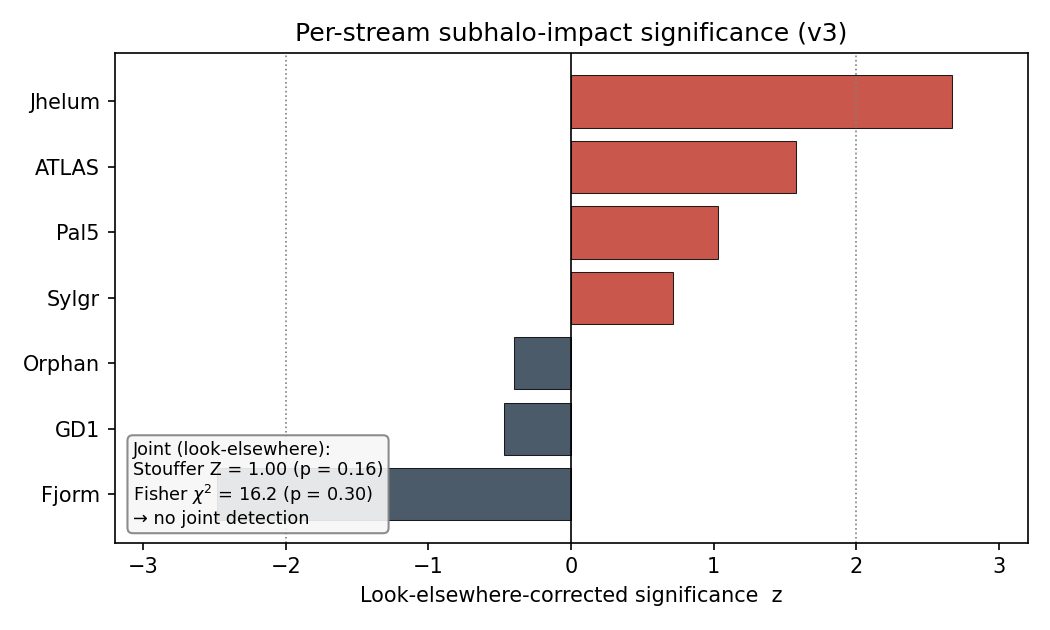
\includegraphics[width=\columnwidth]{figures/significance_v3.png}
\caption{Per-stream look-elsewhere--corrected significance for the seven target
streams (v3 simulations). The joint combination is a non-detection (Stouffer
$Z=1.00$, $p=0.16$; Fisher $\chi^2=16.2$, $p=0.30$).}
\label{fig:sig}
\end{figure}

The combined significance is Stouffer $Z=1.00$ ($p=0.159$) and Fisher
$\chi^2=16.2$ ($p=0.301$) --- no joint detection (Fig.~\ref{fig:sig}). The
per-stream evidence is now coherent and modest, spanning only
$z\in[-2.5,+2.7]$, in contrast to a pre-correction analysis (mixed-sign, 71\%
positive, $z\in[-4.8,+29]$) whose incoherence we attribute to the
simulation-to-observation gap. The corrected simulator both lowers and
regularises the significance; we report a non-detection consistent with a smooth
null --- an upper limit / CDM-consistency given current data and the catalogue
limitations of \S\ref{sec:limits}.

\section{Limitations and systematics}
\label{sec:limits}
\begin{enumerate}
\item Length-versus-width tension in the simple spray (\S\ref{sec:sim}).
\item GD-1 membership contamination; need for an external
  \citet{PriceWhelanBonaca2018}/\textsc{streamfinder} catalogue.
\item A static error-DR profile cache versus fully dynamic per-epoch randomization
  (a speed/fidelity trade).
\item Null-construction confounds (\S\ref{sec:stats}).
\item Forward-model grid resolution and the single-encounter assumption.
\item \textbf{Detection signal strength is dataset-dependent.} Earlier high
  accuracy (AUC~$\approx0.88$--$0.94$) was obtained on a balanced training set; on
  physics-prior datasets cheap baselines reach only AUC~$\approx0.65$--$0.68$.
  Confirmed on v3: AUC~$=0.618$ versus $0.937$ on the balanced set.
\end{enumerate}

\section{Reproducibility}
\label{sec:repro}
The pipeline is public, with a conda environment specification, $\sim$289 unit
tests across 13 files, a categorised script index, and changelogs documenting each
methodological decision. All datasets are regenerable from a single deterministic,
thread-pinned generation script.

\section{Conclusions}
\label{sec:conclusions}
We have built a reproducible pipeline for subhalo-impact detection in stellar
streams and, deliberately, reported what current data and simulations support.
(1)~We diagnosed and partially closed a simulation-to-observation gap (a
track-anchored progenitor IC and error-domain randomization). (2)~On
physically-faithful simulations the detector reaches only AUC~$=0.618$ versus
$0.937$ on a balanced set --- direct evidence that strong reported performance can
be an artefact of training-set construction. (3)~The look-elsewhere--corrected,
coherence-gated multi-stream analysis yields no joint detection (Stouffer
$p=0.16$; Fisher $p=0.30$), consistent with a smooth null / CDM and best read as
an upper limit. The overarching message is that closing the sim-to-real gap
\emph{raises} the bar for claimed detections, and that reproducible methodology ---
including the willingness to report null results --- is essential for turning
stellar streams into a quantitative dark-matter probe. Future work: a
correctly-correlated \citet{Fardal2015} release, an external GD-1 membership
catalogue, and a structure-preserving null for the headline significance.

\section*{Acknowledgements}
This work made use of \textsc{galpy} \citep{Bovy2015galpy}, \textsc{galstreams}
\citep{Mateu2023galstreams}, the \textsc{sbi} toolkit
\citep{Tejero-Cantero2020sbi}, and public data from Gaia DR3
\citep{GaiaDR3_2023}, S$^5$ \citep{Li2019s5}, and APOGEE
\citep{Majewski2017apogee}.

\section*{Data Availability}
All code and configuration are available in the project repository. The training
simulations are regenerable from the provided scripts; public survey data are
available from their respective archives.

\bibliographystyle{mnras}
\bibliography{references}

\bsp
\label{lastpage}
\end{document}
